\documentclass{article}
\usepackage{tikz}
\usetikzlibrary{shapes.geometric}

\begin{document}

\begin{figure}[h]
    \centering
    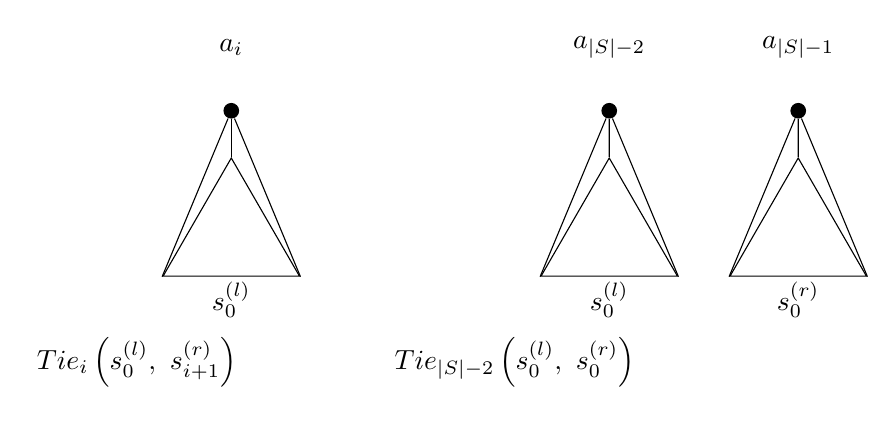
\begin{tikzpicture}[scale=0.8]
        % Left side
        \node[regular polygon, regular polygon sides=3, draw, minimum size=2cm] (triangle1) at (0,0) {};
        \node[circle, fill, inner sep=2pt] (root1) at (0,2) {};
        \draw (triangle1.corner 1) -- (root1);
        \draw (triangle1.corner 2) -- (root1);
        \draw (triangle1.corner 3) -- (root1);
        
        \node at (0, -1) {$s_0^{(l)}$};
        \node at (0, 3) {$a_i$};
        
        \node at (-1.5,-2) {$Tie_i\left(s_0^{(l)},\ s_{i+1}^{(r)}\right)$};
        
        % Right side
        \node[regular polygon, regular polygon sides=3, draw, minimum size=2cm] (triangle2) at (6,0) {};
        \node[regular polygon, regular polygon sides=3, draw, minimum size=2cm] (triangle3) at (9,0) {};
        \node[circle, fill, inner sep=2pt] (root2) at (6,2) {};
        \node[circle, fill, inner sep=2pt] (root3) at (9,2) {};
        \draw (triangle2.corner 1) -- (root2);
        \draw (triangle2.corner 2) -- (root2);
        \draw (triangle2.corner 3) -- (root2);
        
        \draw (triangle3.corner 1) -- (root3);
        \draw (triangle3.corner 2) -- (root3);
        \draw (triangle3.corner 3) -- (root3);
        
        \node at (6, -1) {$s_0^{(l)}$};
        \node at (9, -1) {$s_0^{(r)}$};
        
        \node at (6, 3) {$a_{|S|-2}$};
        \node at (9, 3) {$a_{|S|-1}$};
        
        \node at (4.5,-2) {$Tie_{|S|-2}\left(s_0^{(l)},\ s_0^{(r)}\right)$};
    \end{tikzpicture}
\end{figure}

On the left-hand side we can see an illustration of how the trees in $\mathcal{T}_i$ can be decomposed for $i \in \mathcal{I}_{|S|-2}$, and on the right-hand side we can see how the trees in $\mathcal{T}_{|S|-2}$ can be decomposed.

\end{document}